\section{Creating a Data Package } \label{sec:creating}

When you create a data package in Morpho, you begin by entering data
about the entire data set (e.g., title, abstract, and contact
information). This summary information is the \emph{minimum} amount of
documentation necessary for creating a data package, and can be compiled
using Morpho's \hyperref[sec:wizard-newdp]{Data Package wizard}.

Once the entire data set has been described using the Data Package
wizard, you can begin adding information about the data objects
themselves (i.e., information about the individual data tables, such as
column names and measurement scales). Information about individual data
objects is compiled using Morpho's \hyperref[sec:wizard-newtable]{Data
Table wizard}. 

After the data set has been fully documented, choose whether or not to
include the data itself in the data package. Including the data and
sharing it on the network allows you to take advantage of DataONE 
replication features, which ensure that your data is secure.

\subsection{Opening the New Data Package Wizard} \label{sec:wizard-newdp}

The easiest way to start creating a data package is with Morpho's Data
Package wizard, a handy and powerful tool for collecting general
information that applies to an entire data set. General information
includes: title and abstract, keywords, people and organizations, usage
rights, research project information, spatial coverage information,
methods and sampling information, and access information. 

The Data Package wizard walks you through the process of creating
metadata in a straightforward 15-step process. If you need to stop
working during this process and would like to resume later, see the
\nameref{sec:dp-saveforlater} section.

To open the wizard and begin creating a data package, do one of the
following:
\begin{itemize}
  \setlength{\parskip}{1pt}
  \item click the New Data Package button
    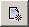
\includegraphics[scale=0.7]{images/button-new-dp.png} found on the
    in the \nameref{sec:toolbar}
  \item click ``Create a New Data Package\ldots'' on the
    \hyperref[sec:panel-work]{main Morpho screen}
  \item select ``New Data Package'' from the \nameref{sec:menu-file}
\end{itemize}

The Data Package Wizard generates a data package based on the entered
information. 

Use the following key-board shortcuts to navigate through the wizard.
\begin{itemize}
  \setlength{\parskip}{1pt}
  \item left and right arrows take you forward and back through the
    wizard steps. Note that if the cursor is in a text field, left and
    right arrows move the cursor left and right inside that field.
  \item ``Esc'' exits the wizard
  \item ``Tab'' moves from one field to the next. Note that for some
    text-entry fields (e.g., abstract), the Tab key inserts a tab.
  \item ``Enter'' skips to the next step in the wizard
\end{itemize}

\subsection{Adding Metadata to the Package} \label{sec:adding-metadata}

The Data Package wizard (\autoref{fig:wizard-dp-introduction.jpg}) helps
you gather the minimum amount of documentation necessary for creating a
data package:
\begin{itemize}
  \setlength{\parskip}{1pt}
  \item \nameref{sec:wizard-dp-title}
  \item \nameref{sec:wizard-dp-keywords}
  \item \nameref{sec:wizard-dp-people}
  \item \nameref{sec:wizard-dp-project}
  \item \nameref{sec:wizard-dp-usage}
  \item \nameref{sec:wizard-dp-coverage} (geographic, temporal,
    taxonomic)
  \item \nameref{sec:wizard-dp-methods}
  \item \nameref{sec:wizard-dp-access}
  \item \nameref{sec:wizard-dp-summary}
\end{itemize}

Required fields are identified with red labels. You must fill out all
required fields before proceeding to the next step. Remember, you can
always change the documentation at a later time using items in the  
\nameref{sec:menu-documentation}.

The wizard displays instructions for filling out each screen. We
recommend that you read the explanatory text before filling out the
wizard forms.

\begin{figure}
  \centering
    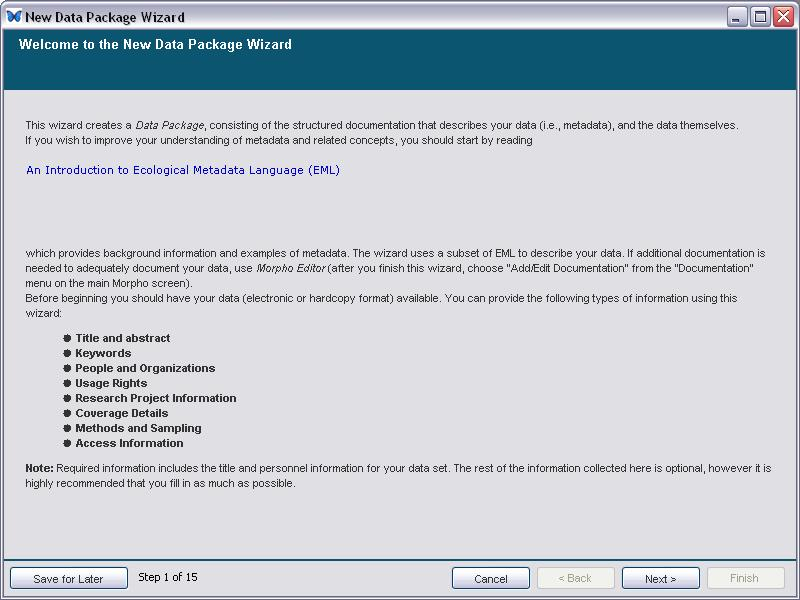
\includegraphics[width=0.7\textwidth]{images/wizard-dp-introduction.jpg}
  \caption{The first screen (Step 1) of Morpho's Data Package Wizard.}
  \label{fig:wizard-dp-introduction.jpg}
\end{figure}
 

\subsubsection{Title and Abstract} \label{sec:wizard-dp-title}

The second step of the Data Package Wizard
(\autoref{fig:wizard-dp-title}) collects a data set title (required) and
abstract. The title provides a full description of the package, and
should be detailed enough to differentiate the package from other
similar data packages. The abstract consists of a paragraph or more
describing the data. Although the abstract is optional, it is very
useful, and we highly recommended that you include an abstract with your
package documentation.

Type the title and abstract directly into the fields, or create them
elsewhere and paste them into the appropriate spots. Use the keyboard
shortcuts ``control+C'' for copy and ``control+V'' for paste. 
Character encoding differences can create problems when cutting and pasting 
special characters from other applications into Morpho. Morpho uses UTF-8 
character encoding.

EML 2.1.1 can accommodate translations for critical metadata. Translations can
be added and edited using the translation editor window 
(\autoref{fig:wizard-dp-title-translations}) accessed by clicking the Translations button. 
The language for the translation should be specified using a valid ISO language 
code and optional ISO country code separated by a dash (i.e. 'en-US').

\begin{figure}
  \centering
    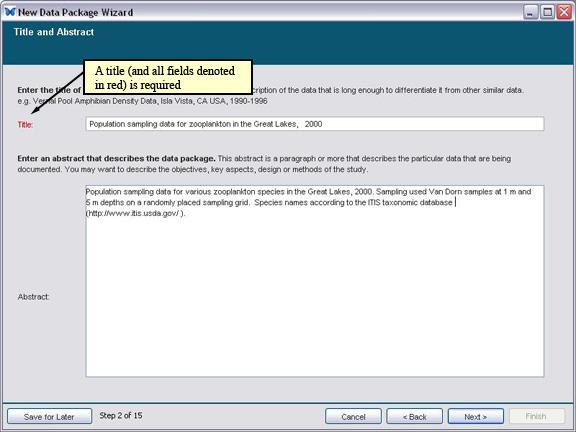
\includegraphics[width=0.7\textwidth]{images/wizard-dp-title.jpg}
  \caption{Step 2 of the Data Package Wizard. Add a title (required) and
    abstract.}
  \label{fig:wizard-dp-title}
\end{figure}

\begin{figure}
  \centering
    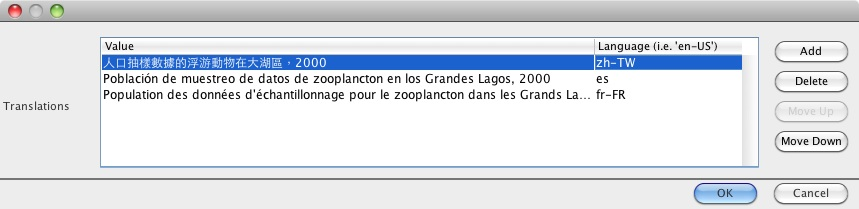
\includegraphics[width=0.7\textwidth]{images/wizard-dp-title-translations.jpg}
  \caption{Data Package Wizard Translations. Add title translations.}
  \label{fig:wizard-dp-title-translations}
\end{figure}

\subsubsection{Keywords} \label{sec:wizard-dp-keywords}

Keywords -- significant words or phrases that help identify the data set
-- are specified in Step 3 of the Data Package wizard
(\autoref{fig:wizard-dp-keywords}) By entering keywords, you enable your
data packages to be easily searched and categorized. If you wish, you
can use keywords from a predefined list (such as the
\href{http://thesaurus.nbii.gov/portal/server.pt}{NBII Biocomplexity
Thesaurus} or KNBRegistry thesaurus, which allows data managers to
select an organizational affiliation for a given data set) that
associates an authoritative definition with the terms. 

\begin{figure}
  \centering
    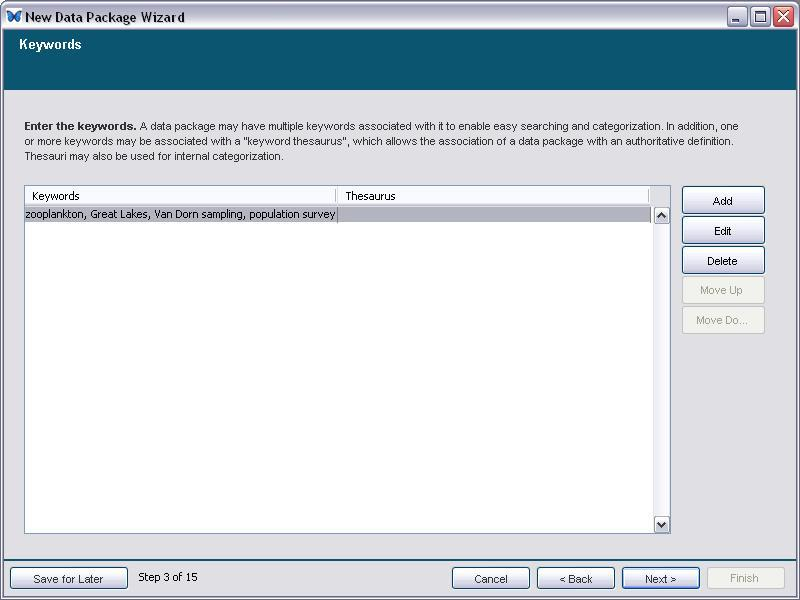
\includegraphics[width=0.7\textwidth]{images/wizard-dp-keywords.jpg}
  \caption{Step 3 of the Data Package wizard displaying example
    keywords.}
  \label{fig:wizard-dp-keywords}
\end{figure}

To add a new set of keywords, click ``Add'' to open the ``Define Keyword
Set'' screen (\autoref{fig:wizard-dp-keywords-fromlist}). Click the
``Add'' button on the Define Keyword Set screen to add a keyword to the
list. To delete a keyword, select it and click ``Delete.''  Use the
``Move Up'' and ``Move Down'' buttons to alter the order of the
keywords. If the keywords are selected from a predefined list, click the
radio button beside ``These keywords are chosen from a predefined list''
and select the name of the thesaurus 
(\href{http://thesaurus.nbii.gov/portal/server.pt}{NBII Biocomplexity
Thesaurus} or KNBRegistry thesaurus) from the drop-down menu. 

The KNBRegistry thesaurus is only relevant to NCEAS, SAEON and SANParks
data managers, and allows these data managers to select an
organizational affiliation for a given data set. In the case of the
SAEON and SANParks, the thesaurus is used to filter search results for
different locations throughout the park network. The NCEAS entry is also
instrumental for documenting data packages that come from various
working groups hosted by the center.

\begin{figure}
  \centering
    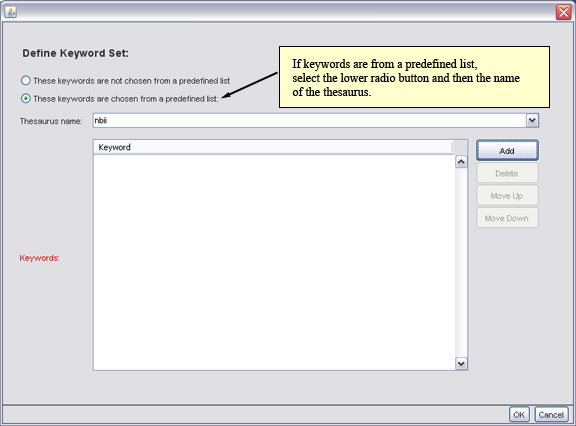
\includegraphics[width=0.7\textwidth]{images/wizard-dp-keywords-fromlist.jpg}
  \caption{Define a keyword set. If the keywords are from a predefined
    list such as a thesaurus, select the lower radio button and the name
    of the thesaurus.}
  \label{fig:wizard-dp-keywords-fromlist}
\end{figure}

Click ``OK'' when you are done adding keywords. The new keywords will
populate the wizard's Step 3 screen (as they appear in
\autoref{fig:wizard-dp-keywords}). To add another, entirely separate
list of keywords -- perhaps for keywords specific to the project --
click ``Add'' and enter a new list of keywords on the Define Keyword Set
screen. Click Next to proceed to Step 4.

\subsubsection{People and Organizations} \label{sec:wizard-dp-people}

Steps 4 through 7 of the Data Package Wizard help users document the
people and organizations responsible for creating the data set, as well
as whom to contact with questions regarding the use or interpretation of
the data. There are three types of people to document:
\begin{description}
  \setlength{\parskip}{1pt}
  \item [Creator] (\emph{required}) The person(s) or organization(s) credited with
    creating the data (e.g., a principle investigator)
  \item [Contact] (\emph{required}) The person(s) or organization(s) to contact
    with questions about use or interpretation of the data. The contact
    may be the same as the creator.
  \item [Associated parties] (\emph{optional}) People or organizations
    functionally associated with the data. For example, the person who
    maintains the database is an associated party with the role of
    'custodian'.
\end{description}

Step 4 simply displays a reminder about what information will be
collected in the following three steps. In Step 5
(\autoref{fig:wizard-dp-creator}), enter information about the data
package creator. Click the Add button to start entering details about each
creator.

\begin{figure}
  \centering
    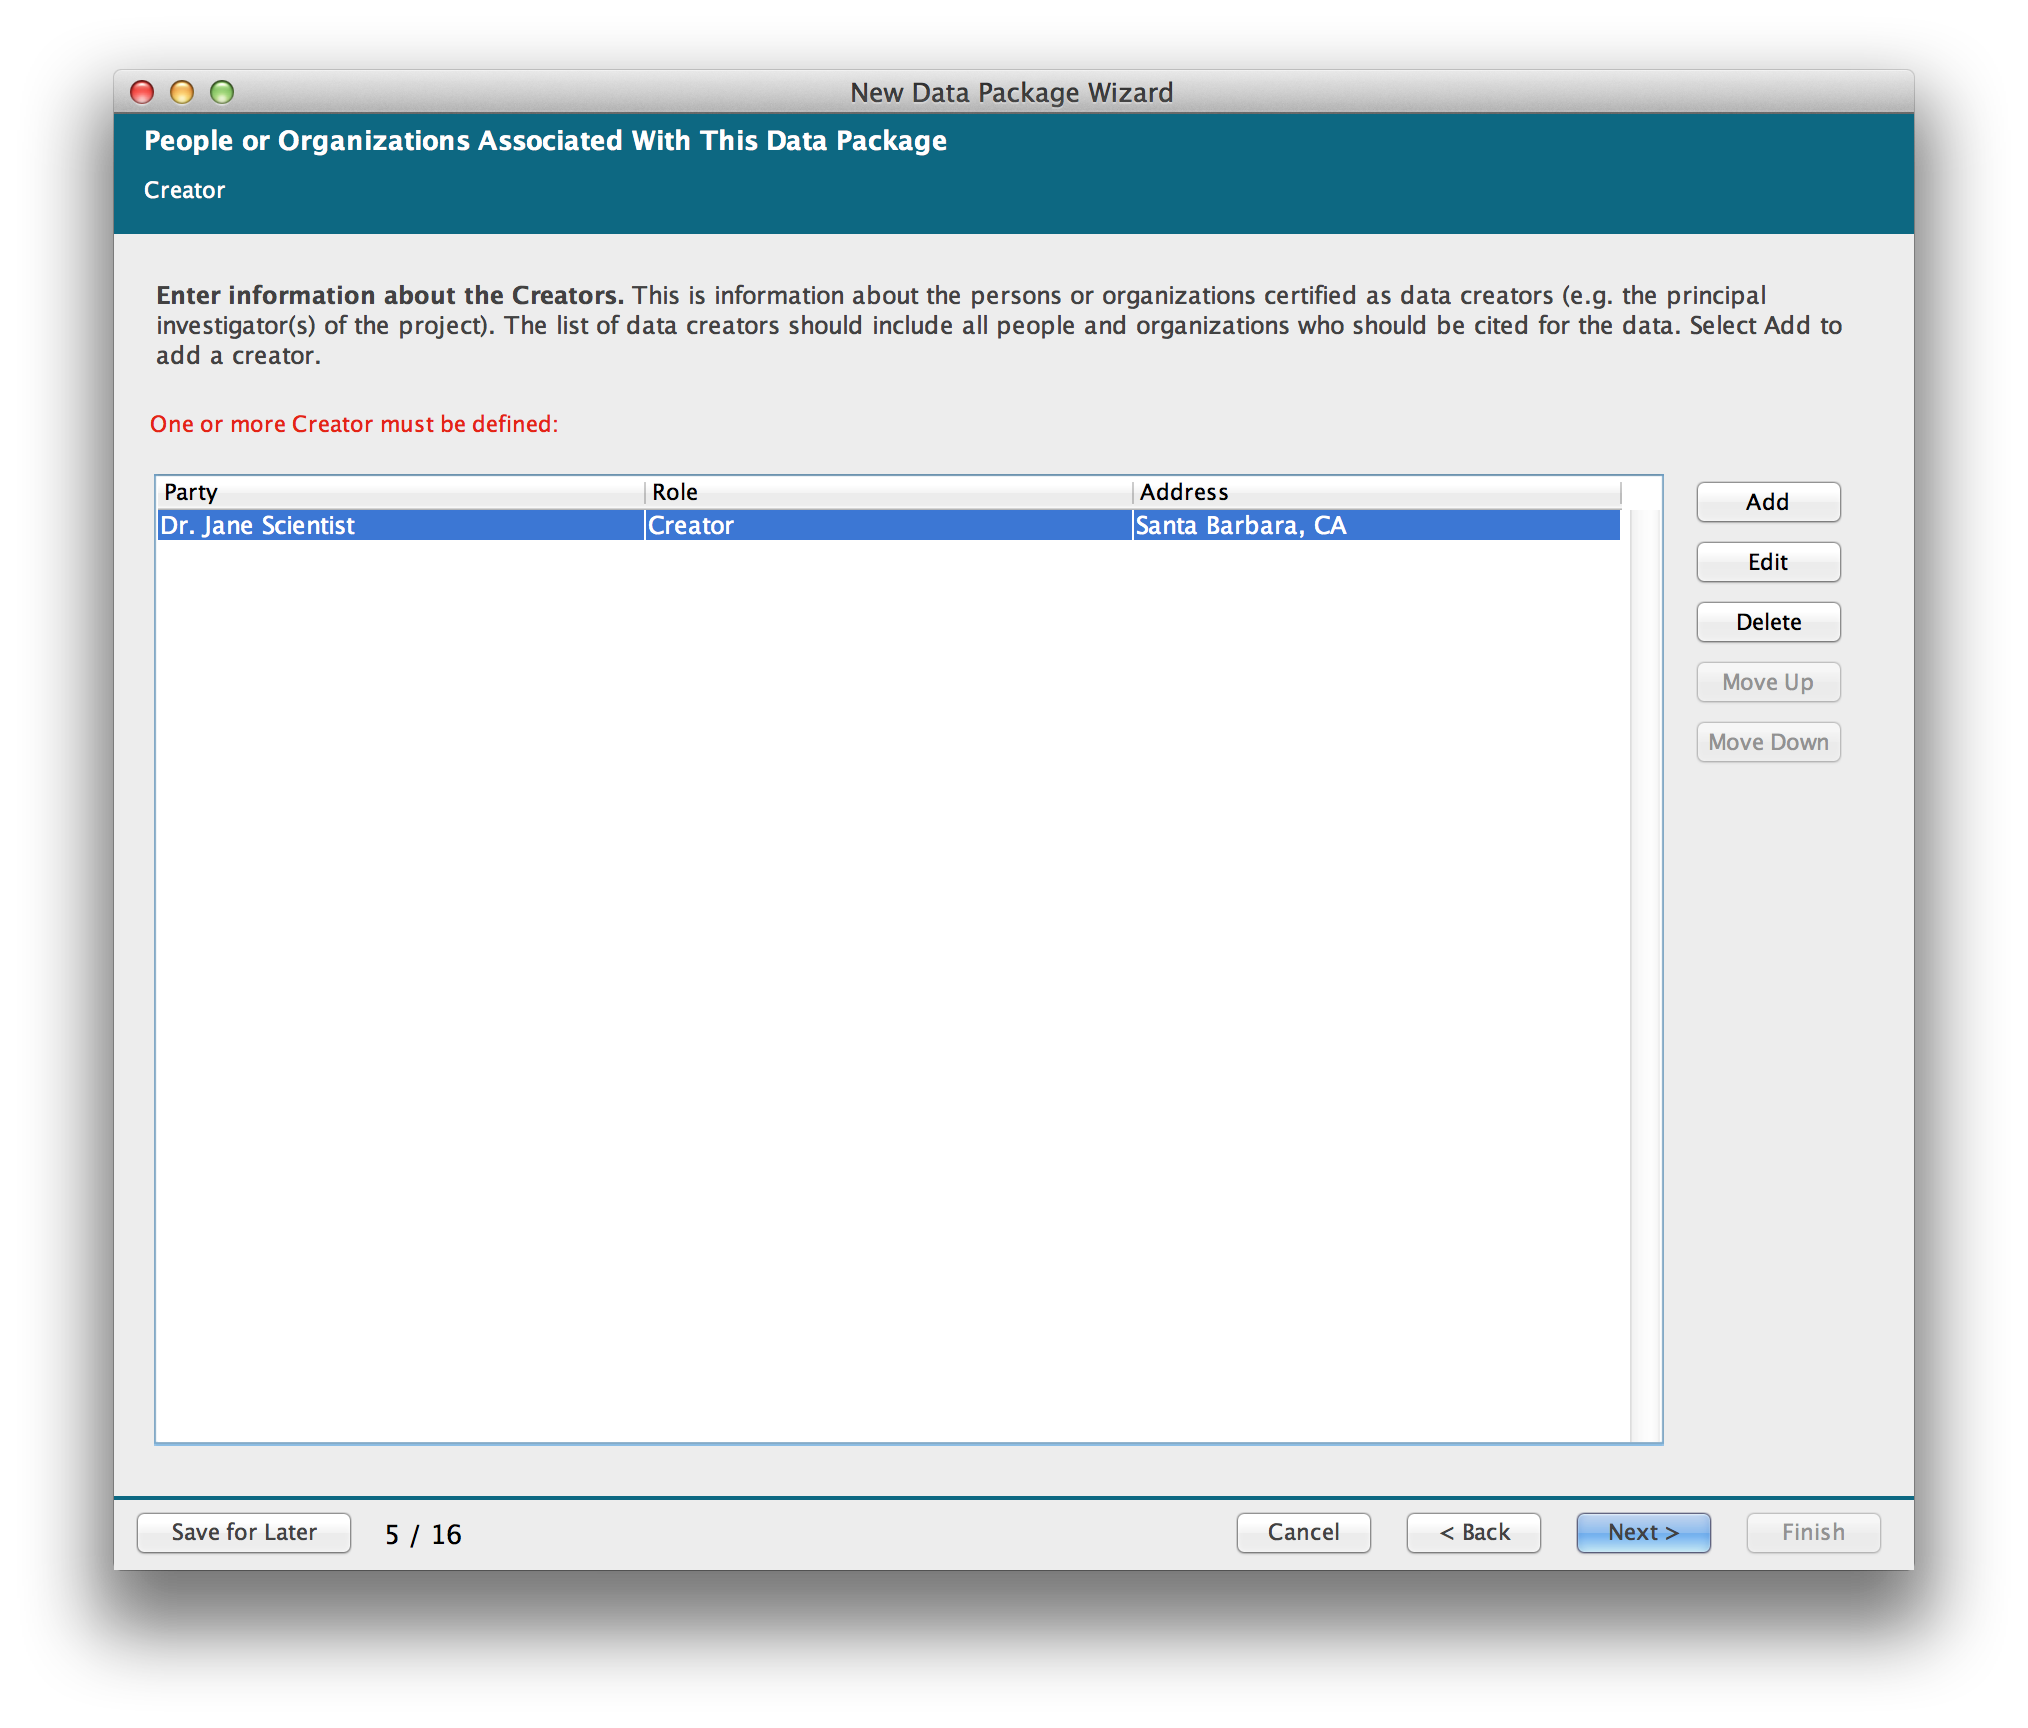
\includegraphics[width=0.7\textwidth]{images/wizard-dp-creator.png}
  \caption{Step 5 of the Data Package Wizard: Click the Add button to
    enter details about the data package creator(s).}
  \label{fig:wizard-dp-creator}
\end{figure}

Enter details about the data set creator in the Creator Details screen
(\autoref{fig:wizard-dp-creator-details}) or populate the form fields with
existing contact information by using the drop-down menu at the top of
the screen. The drop-down menu includes a list of previously entered
data package creators. Select an existing creator to populate the form with
the creator details. Check the ``Do you want to edit the above
information'' check box, and select ``Copy original and edit'' to create
a new set of details based on the existing details. In addition, the
drop-down menu contains an option for viewing a list of all of your
existing data packages and their creators. Select that option to populate
the form fields with information entered in another data package. 

Note: Only one of the three required fields (Last Name, Organization, or
Position Name) must be filled. 

\begin{figure}
  \centering
    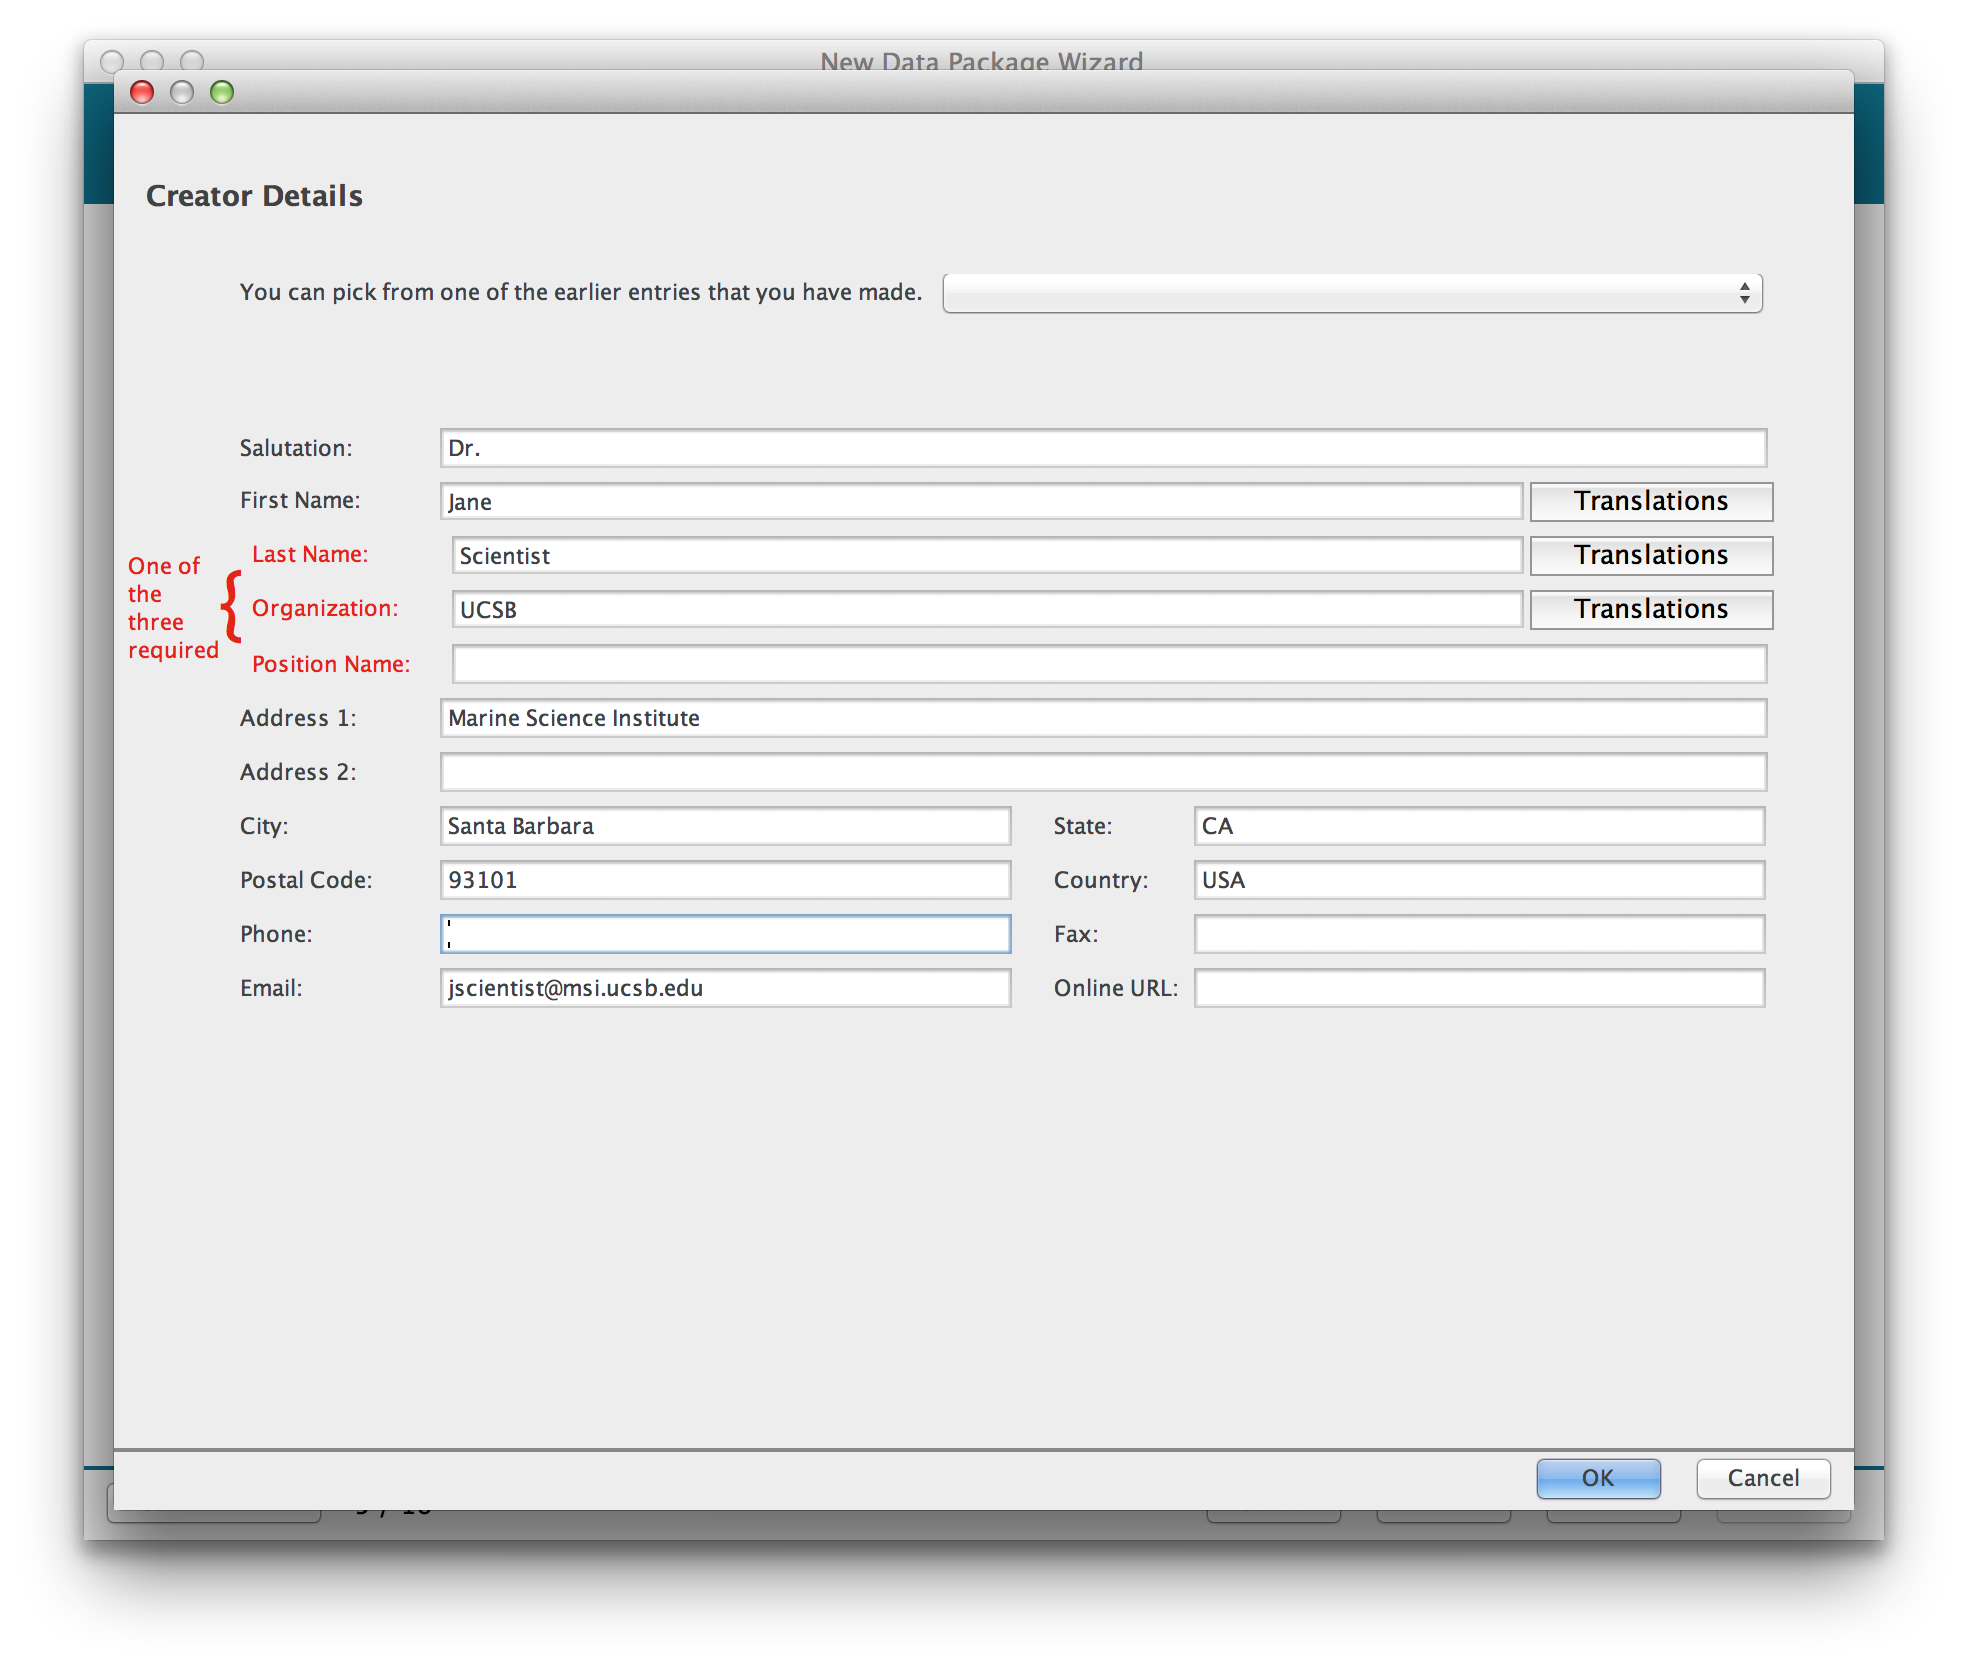
\includegraphics[width=0.7\textwidth]{images/wizard-dp-creator-details.png}
  \caption{Adding details about the data package creator. Note that either
    the creator's last name, organization, or position name is required.}
  \label{fig:wizard-dp-creator-details}
\end{figure}

After entering creator details, click OK. The wizard displays the entered
information on the summary screen. Add additional creators, delete listed
creators, edit creator details, or change the order in which the creators are
listed with the buttons on the right of the screen. 

Click Next to move to Step 6, adding contacts. Adding contacts is very
similar to adding creators. Note that the contact may be the same as the
creator, in which case, you can choose the appropriate person or
organization from the drop-down list at the top of the Contact Details
screen. Otherwise, enter the Contact's information in the form provided.

Step 7, adding Associated Parties, is also similar to adding contacts
and creators. In addition to the details provided in the previous two
steps, you must select a 'Role' from the drop-down list on the
Associated Party Details screen (or type in a role that you'd like to
use) (\autoref{fig:wizard-dp-associated-parties}).

\begin{figure}
  \centering
    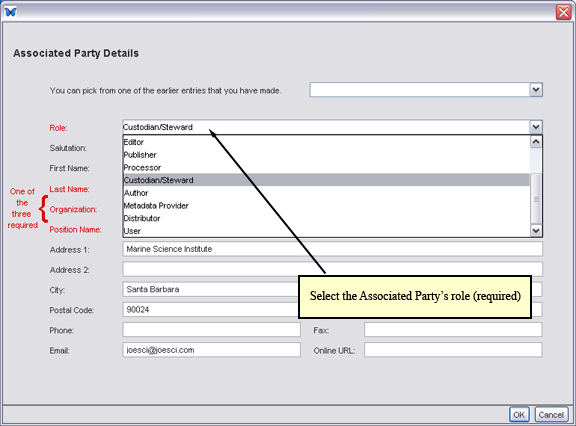
\includegraphics[width=0.7\textwidth]{images/wizard-dp-associated-parties.jpg}
  \caption{Adding Associated Party Details (Step 7 of the Data Package
    Wizard)}
  \label{fig:wizard-dp-associated-parties}
\end{figure}

\subsubsection{Research Project Information} \label{sec:wizard-dp-project}

Data may be associated with a single, independent investigation, or they
may be collected as part of a research program with many sub-projects (a
large NSF grant may provide funds for several investigators to collect
data at various locations, for example). If your data is part of a
larger research project, indicate this by marking the checkbox in Step
8, Research Project Information (\autoref{fig:wizard-dp-project}). You
will be prompted to enter the name of the larger project, its funding
source, and one or more associated people or organizations. 

\begin{figure}
  \centering
    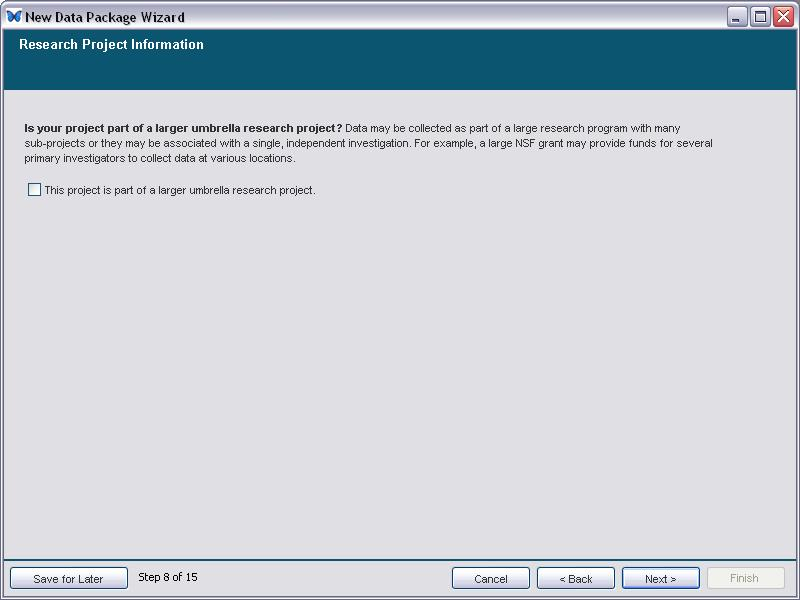
\includegraphics[width=0.7\textwidth]{images/wizard-dp-project.jpg}
  \caption{Step 8 of the Data Package Wizard.}
  \label{fig:wizard-dp-project}
\end{figure}

\subsubsection{Usage Rights} \label{sec:wizard-dp-usage}

Specify the intended usage rights and restrictions (scientific,
technical, ethical) for sharing your data within the public domain
(\autoref{fig:wizard-dp-usage}) in Step 9 of the wizard. You may request
that users inform the Contact person if they wish to use the data
package, for example, or that they read use and access policies that are
posted on a website.

\begin{figure}
  \centering
    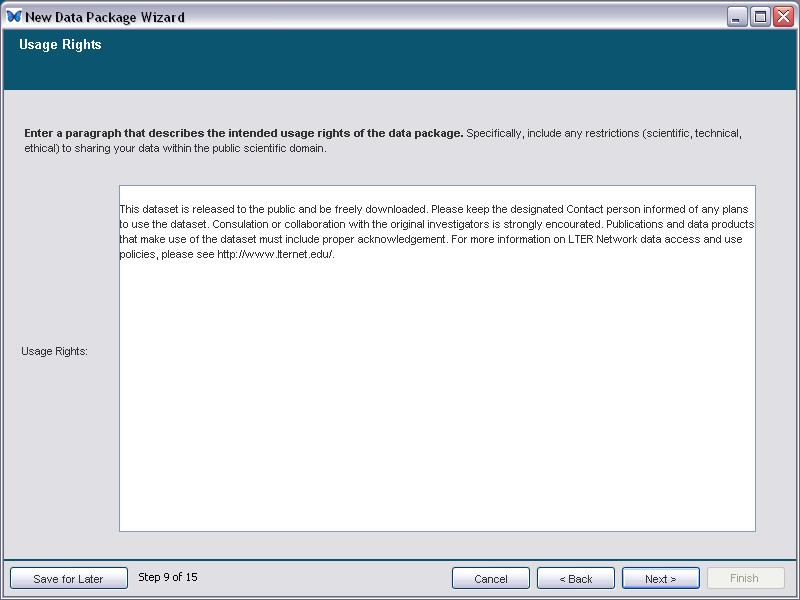
\includegraphics[width=0.7\textwidth]{images/wizard-dp-usage.jpg}
  \caption{Enter the usage rights and restrictions (or copy and paste
    them) into the field provided.}
  \label{fig:wizard-dp-usage}
\end{figure}

Click ``Next'' to move on to Step 10, Coverage Details.

\subsubsection[Coverage Details]{Coverage Details (geographic, temporal,
  taxonomic)} \label{sec:wizard-dp-coverage}

Adding information about the data set's geographic, temporal, and
taxonomic coverage allows users to easily search for data sets by these
criteria. Whether you are documenting the latitude and longitude
coordinates of your study, or specifying the date range over which data
were collected, the wizard's interface simplifies the process by
providing a handy set of data entry tools.

Click the ``Add'' button in Step 10 of the Data Package Wizard
(\autoref{fig:wizard-dp-geographic}), to begin entering information
about the geographic coverage of the data. Coverage can be a single
point (a reserve or park, for example) or a region.

\begin{figure}
  \centering
    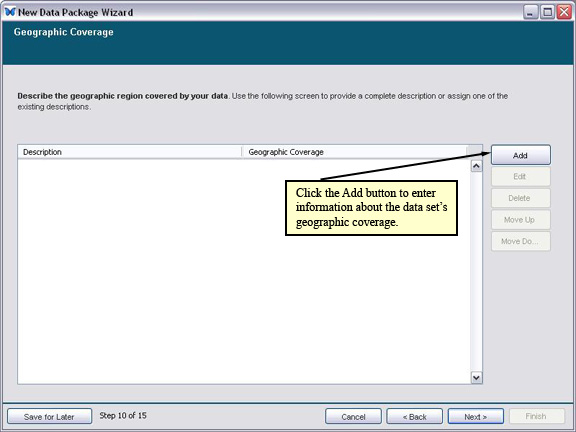
\includegraphics[width=0.7\textwidth]{images/wizard-dp-geographic.jpg}
  \caption{Enter information about the data set's geographic coverage.}
  \label{fig:wizard-dp-geographic}
\end{figure}

After you click the Add button, the Geographic Coverage details screen
opens (\autoref{fig:wizard-dp-geographic-description}).

\begin{figure}
  \centering
    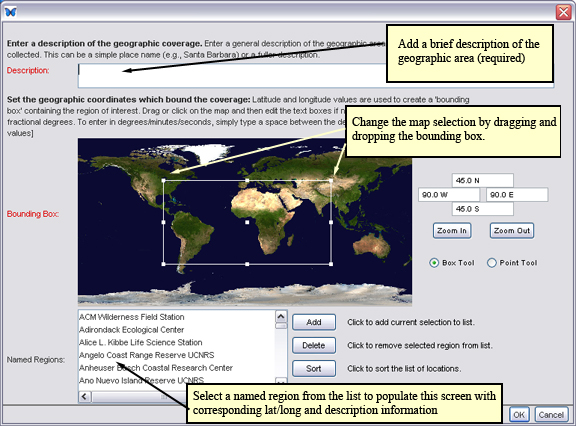
\includegraphics[width=0.7\textwidth]{images/wizard-dp-geographic-description.jpg}
  \caption{Customizing geographic coverage details (step 10 of the Data
    Package wizard).}
  \label{fig:wizard-dp-geographic-description}
\end{figure}

A textual description of the spatial coverage is required. In addition,
you must specify coverage coordinates. To select a geographic region,
use one of the following methods:
\begin{itemize}
  \setlength{\parskip}{1pt}
  \item Select the ``Box Tool'' radio button. Drag the mouse on the map
    to create a selection. Drag the white squares on the edge of the box
    to adjust the edges. 
  \item Select a point on the map by selecting the ``Point Tool'' radio
    button and clicking the map. 
  \item Manually enter latitude and longitude coordinates in the text
    boxes provided.
  \item Select a predefined region or point by selecting a location from
    the named region menu at the bottom of the screen. To add a new
    named region to the list, select the region or point on the map,
    optionally enter a description, and click ``Add''. To remove a named
    region from the list, select the region and click ``Delete''. You
    can also ``Sort'' the items in the list. 
\end{itemize}

Click ``Zoom In'' or ``Zoom Out'' to change the view of the map.

The latitude and longitude coordinates for the selected area or point
will be displayed on the right of the screen. By default, values are
specified in fractional degrees. To enter degrees/minutes/seconds, type
a space between each value.

Click OK to return to the main Geographic Coverage screen. From here,
you can choose to add additional geographic coverage documentation, or
edit, delete, or change the order of the geographic descriptions you
have entered. Click Next to proceed to Step 11, Temporal Coverage
(\autoref{fig:wizard-dp-temporal}).
 
\begin{figure}
  \centering
    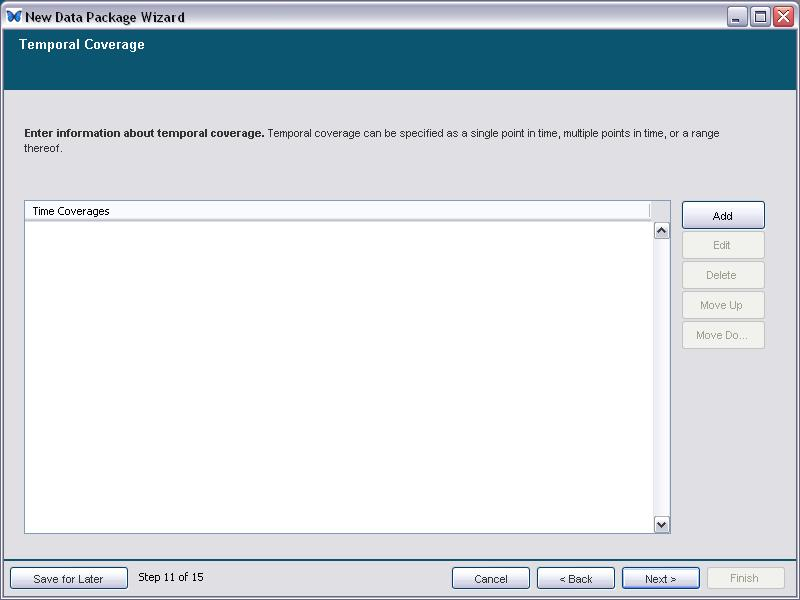
\includegraphics[width=0.7\textwidth]{images/wizard-dp-temporal.jpg}
  \caption{Specify the data set's temporal coverage.}
  \label{fig:wizard-dp-temporal}
\end{figure}

Click the Add button to open the Define Temporal Coverage screen
(\autoref{fig:wizard-dp-temporal-define}).

\begin{figure}
  \centering
    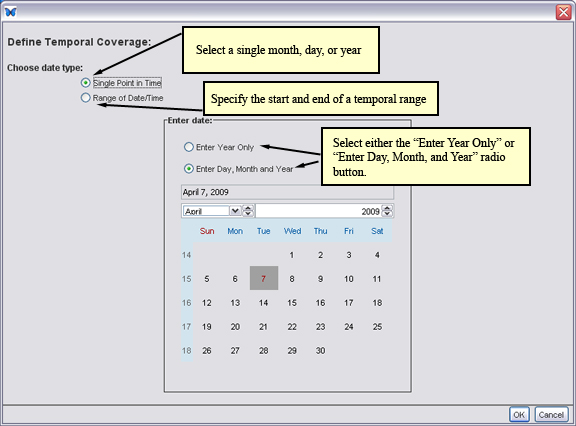
\includegraphics[width=0.7\textwidth]{images/wizard-dp-temporal-define.jpg}
  \caption{Specify temporal coverage details (Step 11 of the Data
    Package wizard).}
  \label{fig:wizard-dp-temporal-define}
\end{figure}

Choose the date type using the radio buttons at the top of the screen:
\begin{itemize}
  \setlength{\parskip}{1pt}
  \item Select ``Single Point in Time'' to specify a temporal coverage
    of a single year or single day. 
  \item Select ``Range of Date/Time'' to specify a start and end date.
    When you select the range radio button, a second calendar will
    appear for collecting end-date information.
\end{itemize}

Select one of the radio button above the calendar to specify only a year
(the default), or a month, year, and day. Select a month and year from
the drop-down menus above the calendars. To select a day, click that day
in the calendar. 

Click OK to return to the main Temporal Coverage screen. Click Next to
proceed to Step 12, Taxonomic Coverage
(\autoref{fig:wizard-dp-taxonomic}).

\begin{figure}
  \centering
    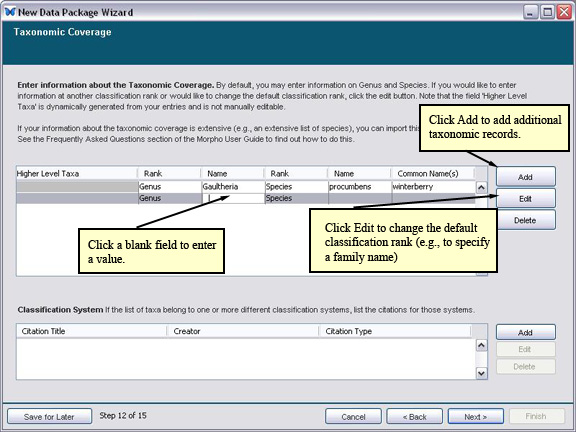
\includegraphics[width=0.7\textwidth]{images/wizard-dp-taxonomic.jpg}
  \caption{Specify taxonomic coverage.}
  \label{fig:wizard-dp-taxonomic}
\end{figure}

The Taxonomic Coverage interface allows you to easily add taxonomic
coverage information for a short list of species (or other taxonomic
ranks). If your data set has a large taxonomic coverage, you will likely
wish to import the data instead of entering it here. This process is
described later in this section.

To add taxonomic coverage for one or two taxon ranks (such as genus and
species, displayed by default), click a blank field beside the rank and
type the corresponding name. Species common name(s) can also be
specified by clicking and typing in the provided field.

To add additional levels of taxonomic information, select a row of
information and click the ``Edit'' button to open the Taxonomic Hierarchy
screen (\autoref{fig:wizard-dp-taxonomic-edit}).

\begin{figure}
  \centering
    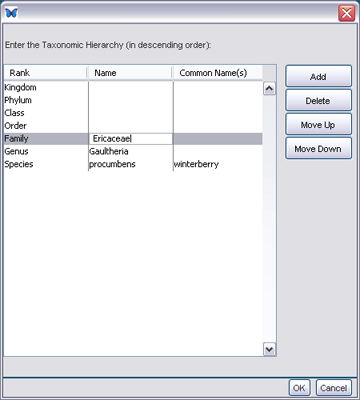
\includegraphics[width=0.7\textwidth]{images/wizard-dp-taxonomic-edit.jpg}
  \caption{Entering the taxonomic hierarchy (for more than two levels).}
  \label{fig:wizard-dp-taxonomic-edit}
\end{figure}

If your taxonomic coverage is extensive, you may wish to import the
information instead of entering it into the wizard. If you chose to
import the taxonomic coverage information, skip Step 12 of the wizard
and complete the remaining wizard steps. You will then need to import
the taxonomic information as a data table and use the ``Import Taxon
Information from Data Table'' option from the Documentation $>$
Taxonomic Coverage menu item to import the list into the appropriate
place. 

To import taxonomic coverage information:
\begin{enumerate}
  \item Save your taxonomic coverage information (e.g., a list of
    species) as a text file.
  \item Open the data package that is associated with the taxonomic
    information.
  \item Select ``Create/Import New Data table'' from the Data menu.
    Click ``IMPORT'' and ``AUTOMATIC'', and locate your species text
    file on your computer. The wizard will display the file.
  \item Complete the \hyperref[sec:adding-data]{Data Table Wizard}. You
    may need to uncheck the space-delimiter box in Step 2 of the wizard
    to display species names in a single column. 
  \item From the Documentation menu, select Taxonomic Coverage. Click
    ``Import Taxon Information from Data table.'' The import screen
    opens (\autoref{fig:wizard-dp-taxonomic-import})
  \item Select the column(s) corresponding to your taxonomic information
    by checking the box at the top of the column. Note that Morpho
    expects species names to be binomials (e.g., Ursus arctos), and so
    the import utility expects to find the binomial in one of the
    imported columns, as shown in
    \autoref{fig:wizard-dp-taxonomic-import}.
  \item A pop up box prompts you to select the taxon rank that
    corresponds to the values in the column. Choose the taxon rank and
    click ``OK''.
  \item Choose to import all of the values in the selected column(s), or
    only certain values using the radio buttons at the bottom of the
    import screen. The two options only apply when the imported taxon
    names are documented as having enumerated values. If this is the
    case, the ``Import all values'' option imports each of the
    predefined codes listed as possible enumerated values (not the
    column values; any taxon value in the column that does not have an
    associated code in the metadata, will not be imported). ``Import
    only values used in the dataset'' imports each unique value in the
    column of data, completely ignoring the codes provided in the
    metadata. Note that because of the way Morpho displays enumerated
    values (with one column containing codes and another their
    definitions), you will not see the column values. If the imported
    column contains free-form text values, both options simply pull in
    the values used in the dataset.
  \item Click Import.
\end{enumerate}

\begin{figure}
  \centering
    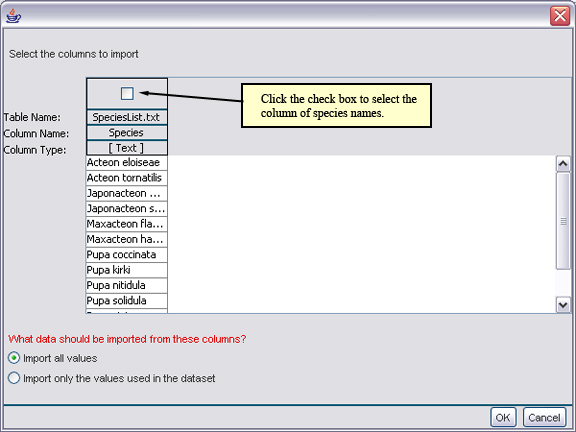
\includegraphics[width=0.7\textwidth]{images/wizard-dp-taxonomic-import.jpg}
  \caption{Importing taxonomic coverage information from a text file.}
  \label{fig:wizard-dp-taxonomic-import}
\end{figure}

Your taxonomic information will appear in the Taxonomic Coverage screen.

\subsubsection{Methods and Sampling} \label{sec:wizard-dp-methods}

Method and sampling information describes the steps followed in
implementing an experiment and the experiment's sampling design (e.g.,
the way in which treatments were assigned to sampling units). Although
this information is not required, it helps other users understand your
data and how it was assembled. Both method and sampling information is
entered in Step 13 of the Data Package Wizard
(\autoref{fig:wizard-dp-methods}).

\begin{figure}
  \centering
    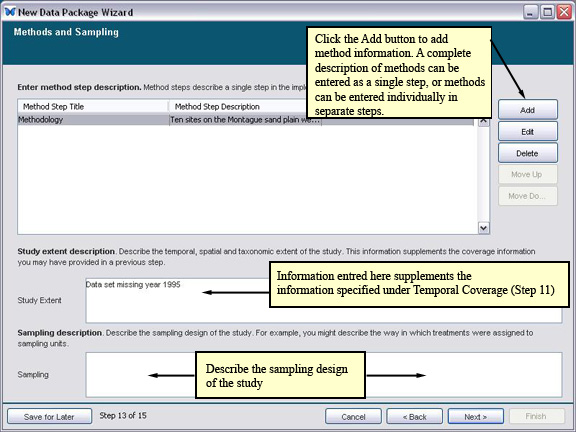
\includegraphics[width=0.7\textwidth]{images/wizard-dp-methods.jpg}
  \caption{Adding information about methods and sampling.}
  \label{fig:wizard-dp-methods}
\end{figure}

To add a method description, click ``Add'' to open the Step Information
screen (\autoref{fig:wizard-dp-methods-step}).

\begin{figure}
  \centering
    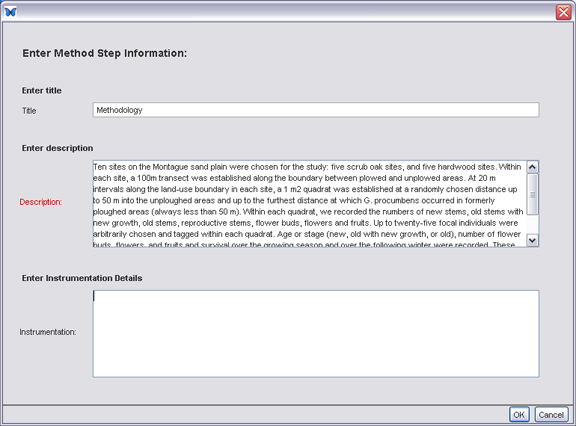
\includegraphics[width=0.7\textwidth]{images/wizard-dp-methods-step.jpg}
  \caption{Entering methodology information.}
  \label{fig:wizard-dp-methods-step}
\end{figure}

Enter a method title (optional), description (required), and
instrumentation details (optional), then click ``OK'' to return to the
main Methods and Sampling screen. 

Study extent information supplements the information already provided in
the temporal or spatial extent of the study. For example, missing years
for temporal coverage should be noted here, or a description of temporal
coverage for data sets beyond the calendar range provided previously
(such as ``the pleistocene'').

Use the sampling description field to provide details on the sampling
design of the study. 

When you have finished entering method and sampling information, click
``Next'' to continue to Step 14 of the wizard, Access Information.

\subsubsection{Access Information} \label{sec:wizard-dp-access}

By setting access information, you control who has access to your data
and metadata (\autoref{fig:wizard-dp-access}). For example, you can
specify that the public can view your data, or that only specified
colleagues can do so. You can also grant specific users and groups
permission to edit your data files, and/or to grant read/edit permission
to additional users. 

By default, the settings specified in the wizard apply to all metadata
and data tables imported into the package. However, after you have added
one or more data tables to the package, you can choose to set different
permissions for each table using the ``Edit Data Table Access'' option in
the Data menu. For example, the data package may permit public read
access, but read access to the data table can be more restrictive (e.g.,
only granted to a specified user group). 

\begin{figure}
  \centering
    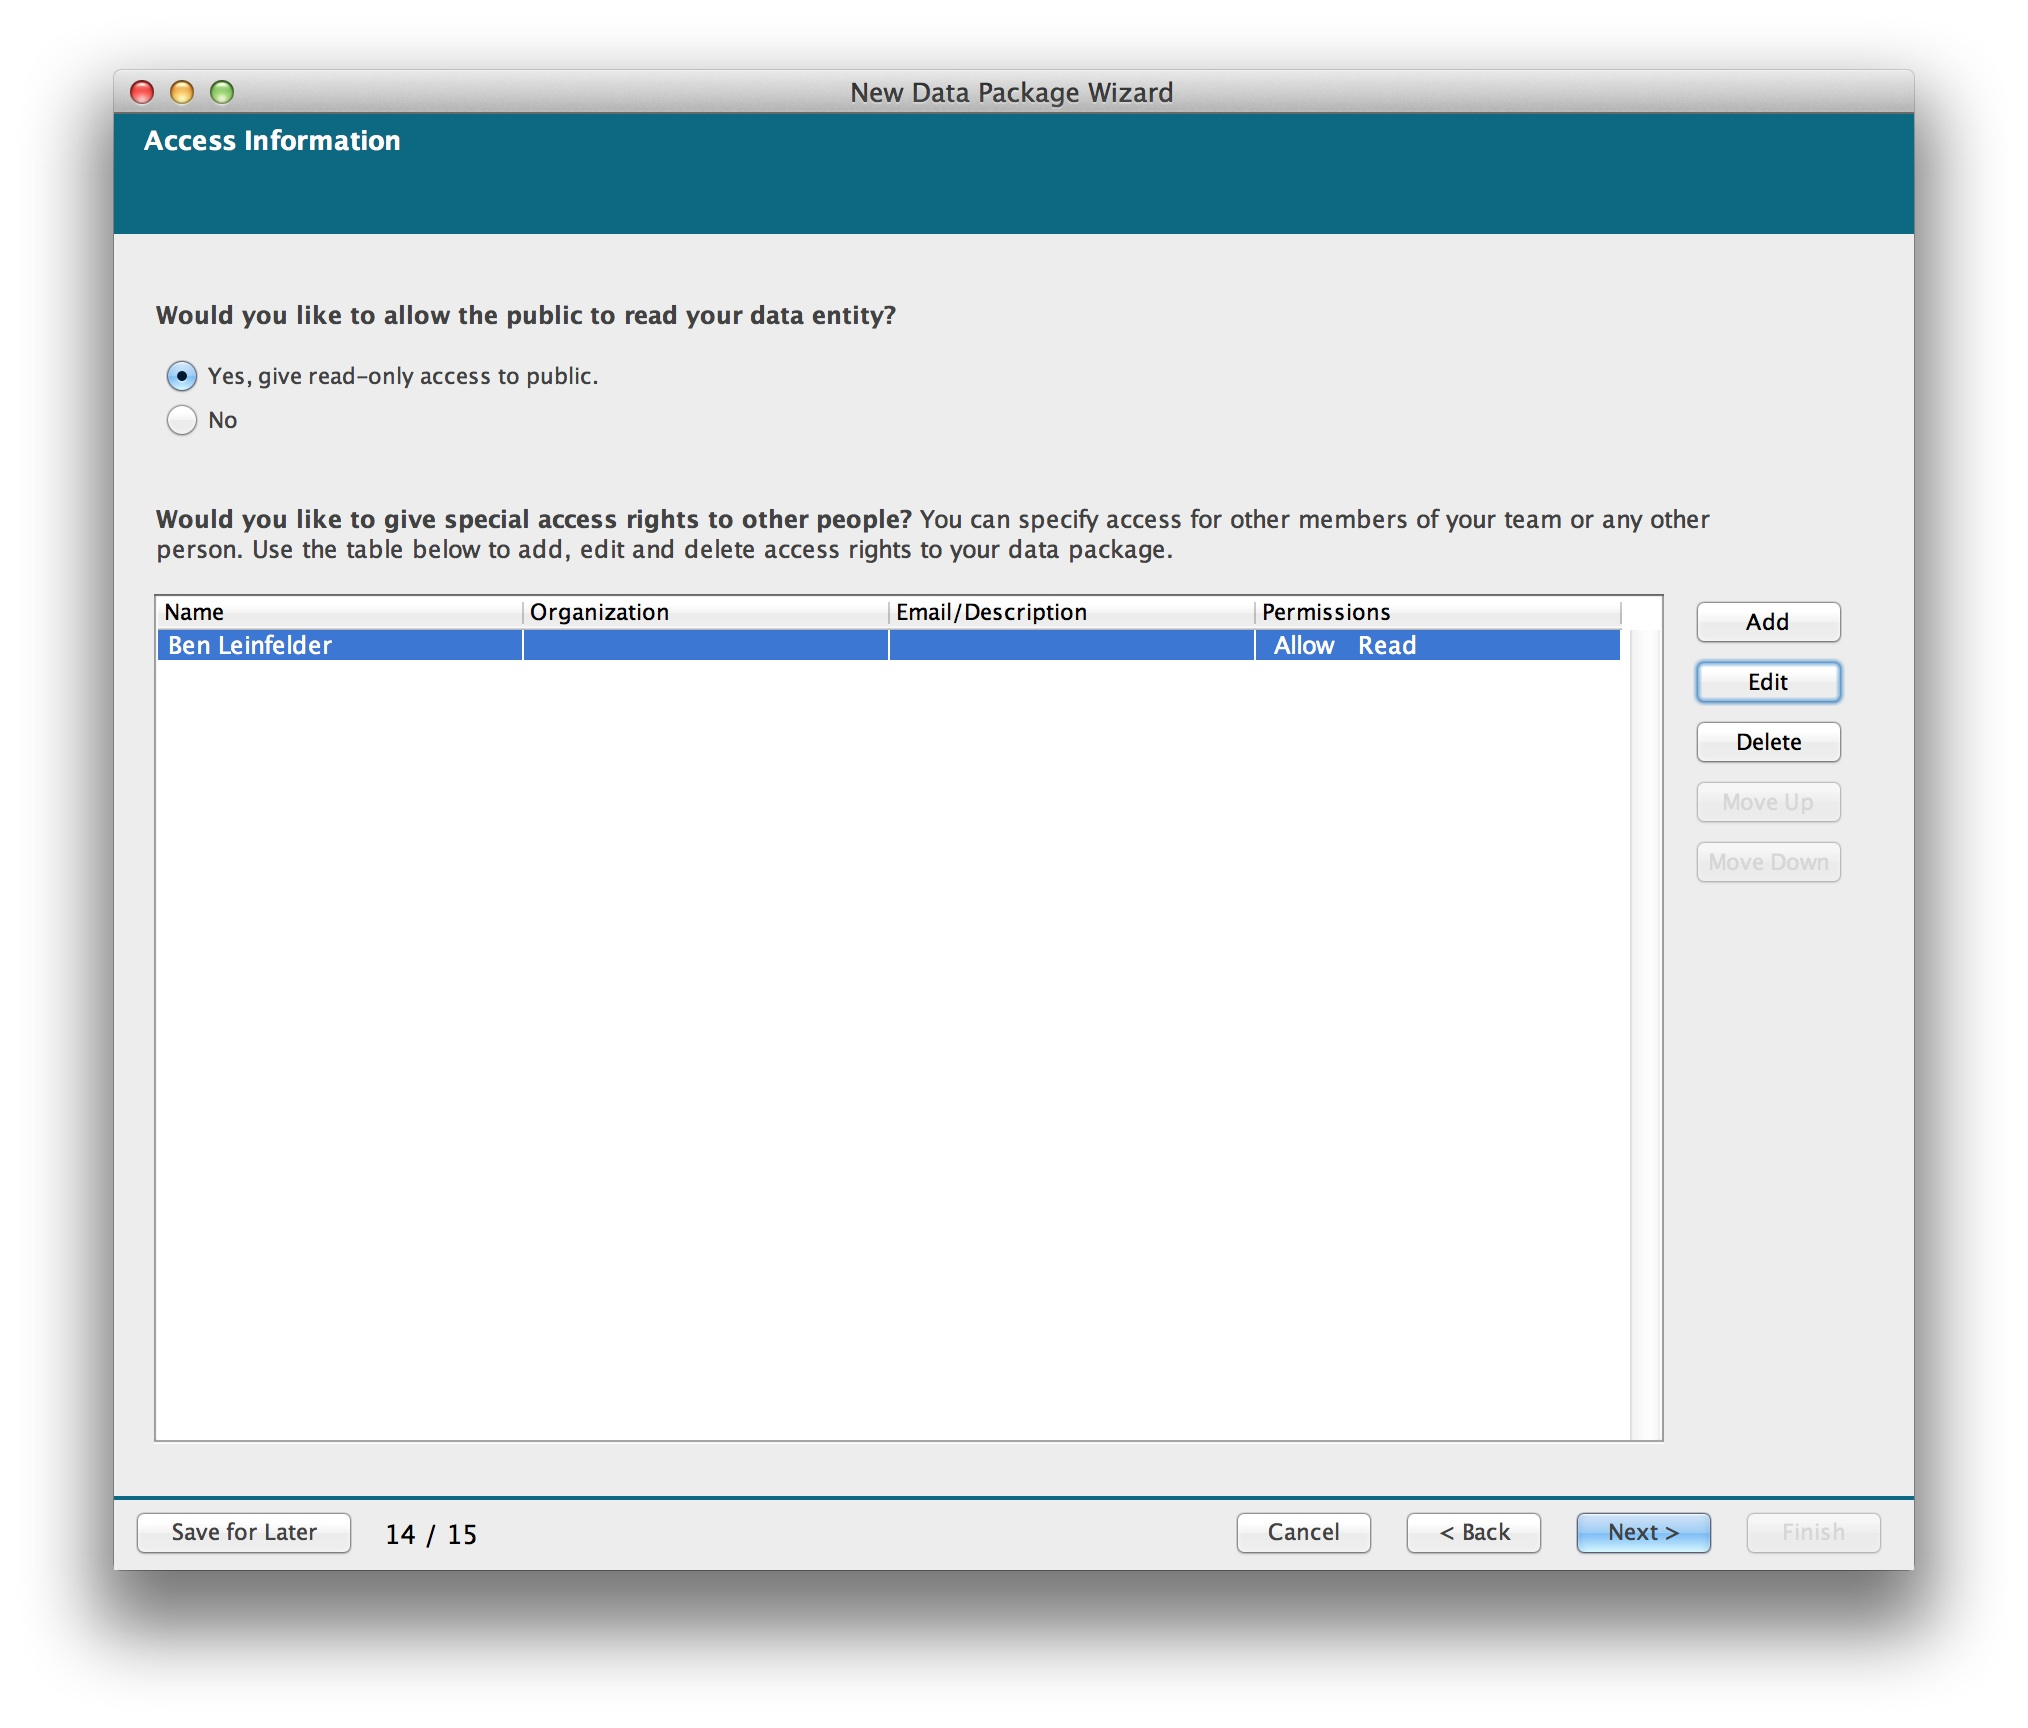
\includegraphics[width=0.7\textwidth]{images/wizard-dp-access.jpg}
  \caption{Set access permissions for the data package.}
  \label{fig:wizard-dp-access}
\end{figure}

Select a radio button from the top of the Access Information screen to
indicate whether or not the public can read your data package once it is
\hyperref[sec:uploading]{placed on a network}.

Click Add to open the Define Access screen
(\autoref{fig:wizard-dp-access-tree}) and grant specific users and
groups customized access to the data package. 

\begin{figure}
  \centering
    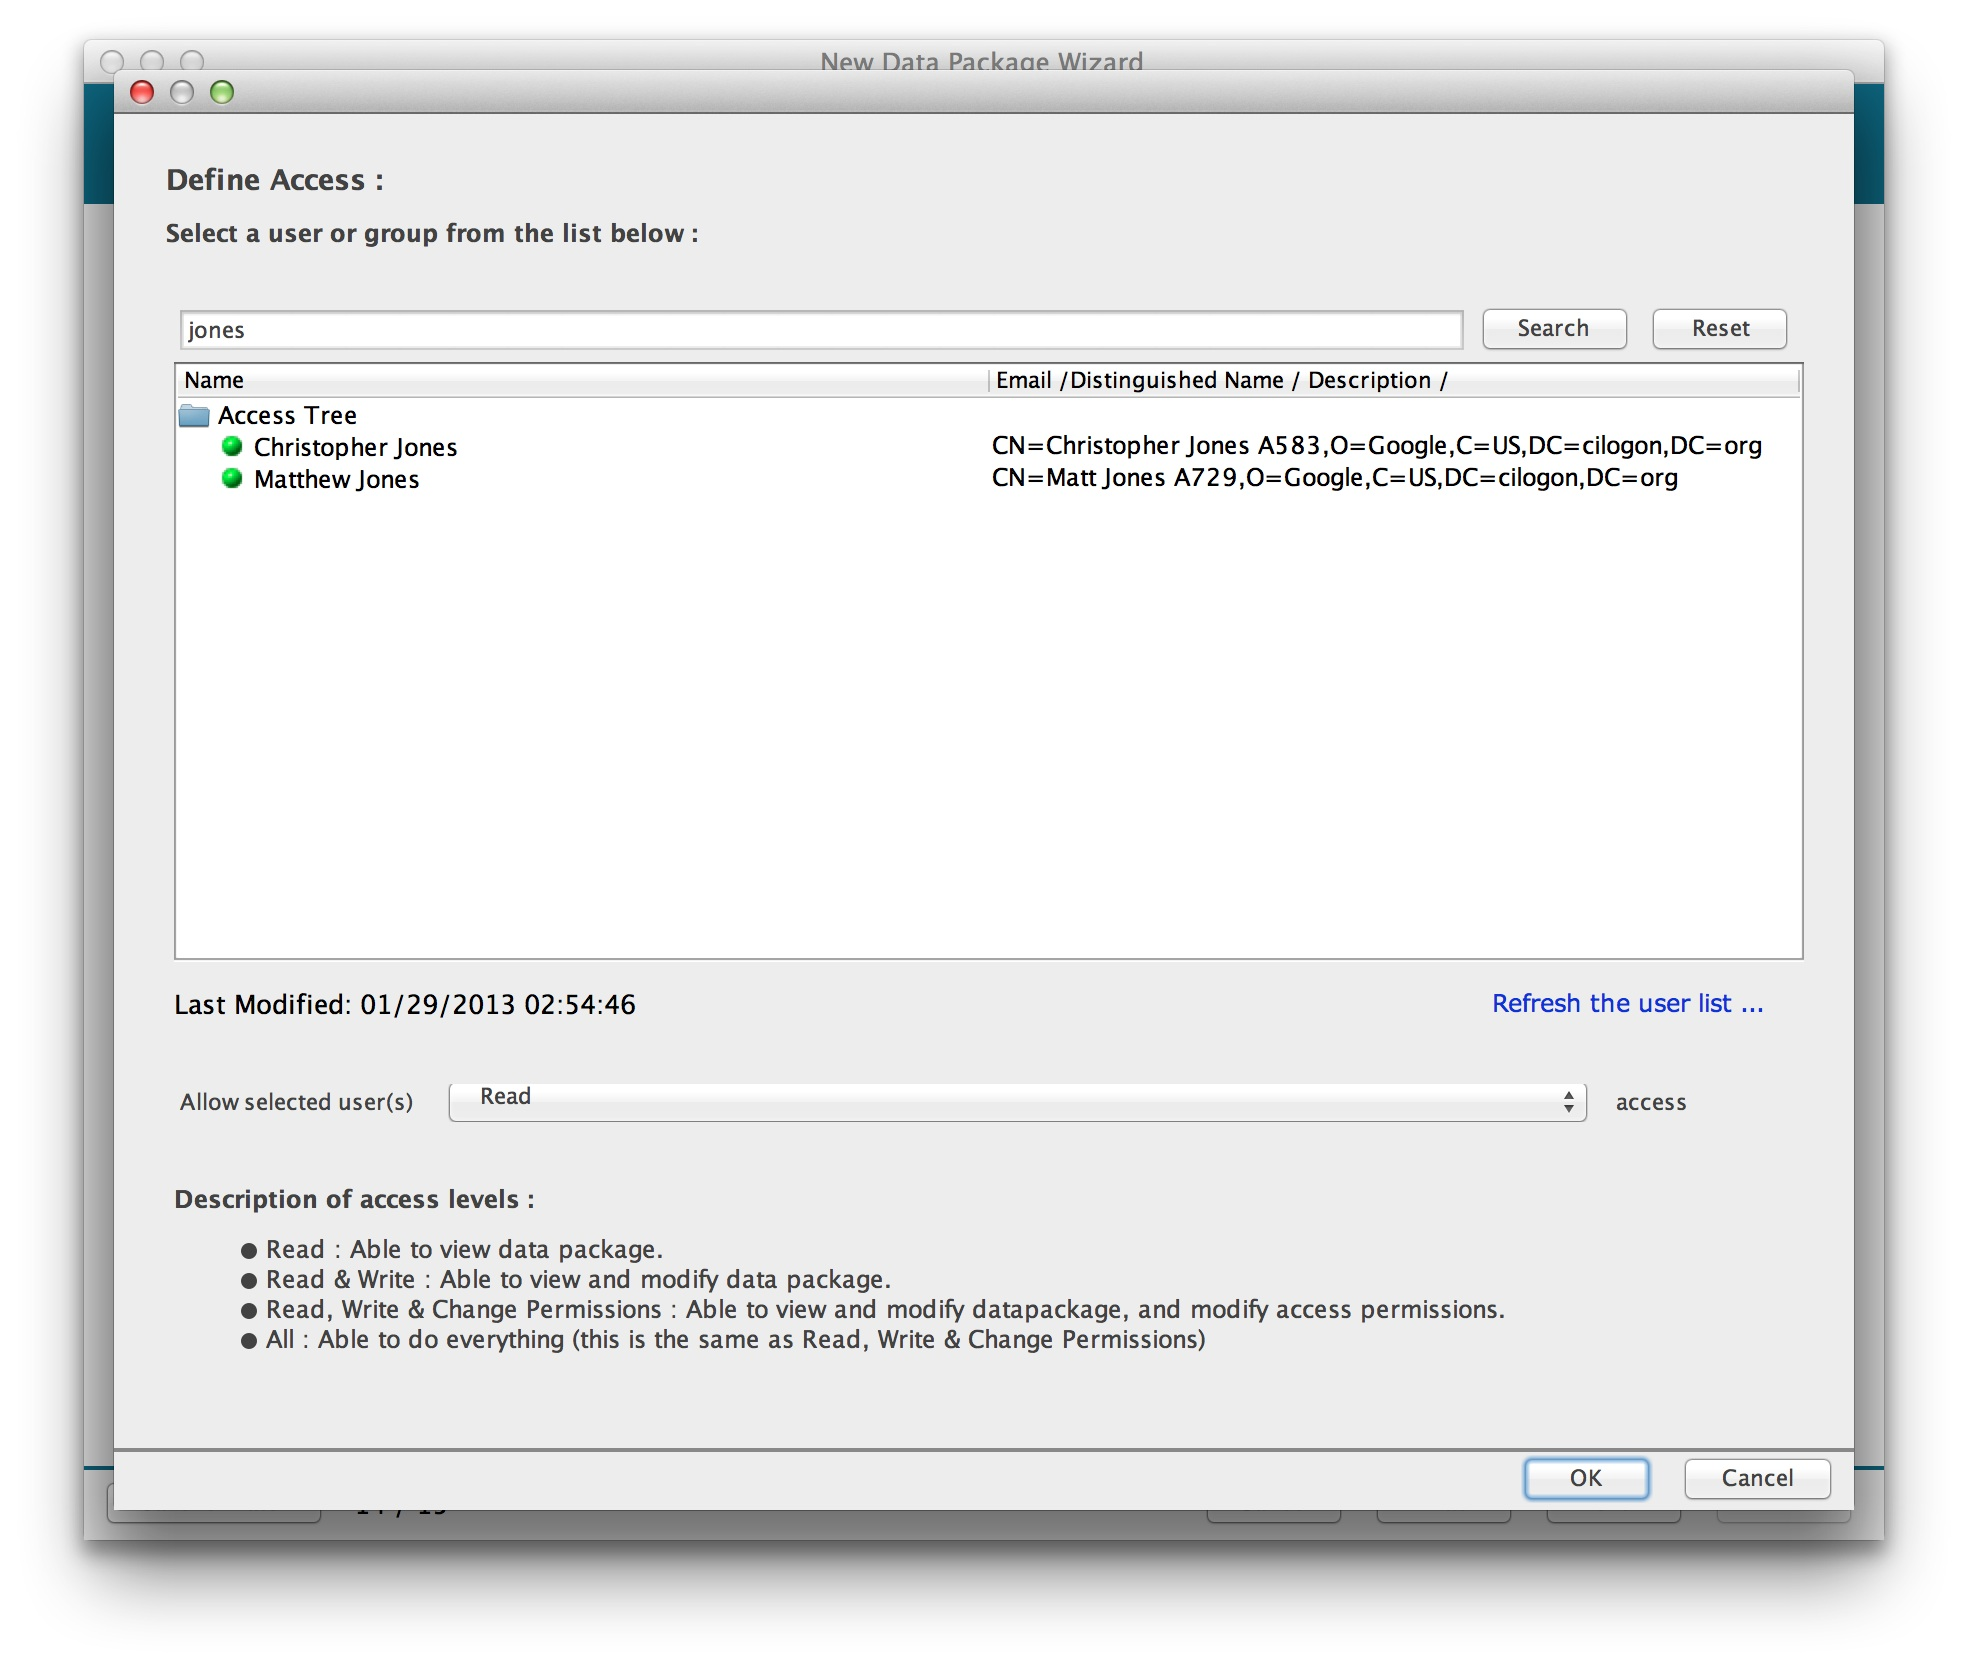
\includegraphics[width=0.7\textwidth]{images/wizard-dp-access-tree.jpg}
  \caption{Select users or user groups and assign appropriate access
    levels.}
  \label{fig:wizard-dp-access-tree}
\end{figure}

After selecting a specific user or user group, define the appropriate
access permissions using the drop-down menus. Choose to Allow access at 
the following levels:
\begin{itemize}
  \setlength{\parskip}{1pt}
  \item Read (able to view the data package)
  \item Read and Write (able to view and modify the data package)
  \item Read and Write and Change Permissions (able to view and modify
    the data package and modify access permissions)
  \item All  (same as Read and Write and Change Permissions)
\end{itemize}

\subsubsection{Replication Policy} \label{sec:wizard-dp-replication}

By specifying a replication policy, you control how your data
and metadata are backed up in the DataONE network (\autoref{fig:wizard-dp-replication}). 
For example, you can specify that 4 copies of the metadata be kept 
at various Member Nodes but that only 2 copies of the data table[s] be stored elsewhere.

Like the access rules, replication policies specified in the wizard apply 
to all metadata and data tables subsequently imported into the package. 
You can choose to set a different replication policy for each table using 
the ``Edit Replication Policy'' option in
the Data menu. For example, you may want a specific Member Node to house a 
large data object because there is surplus space at that node.

\begin{figure}
  \centering
    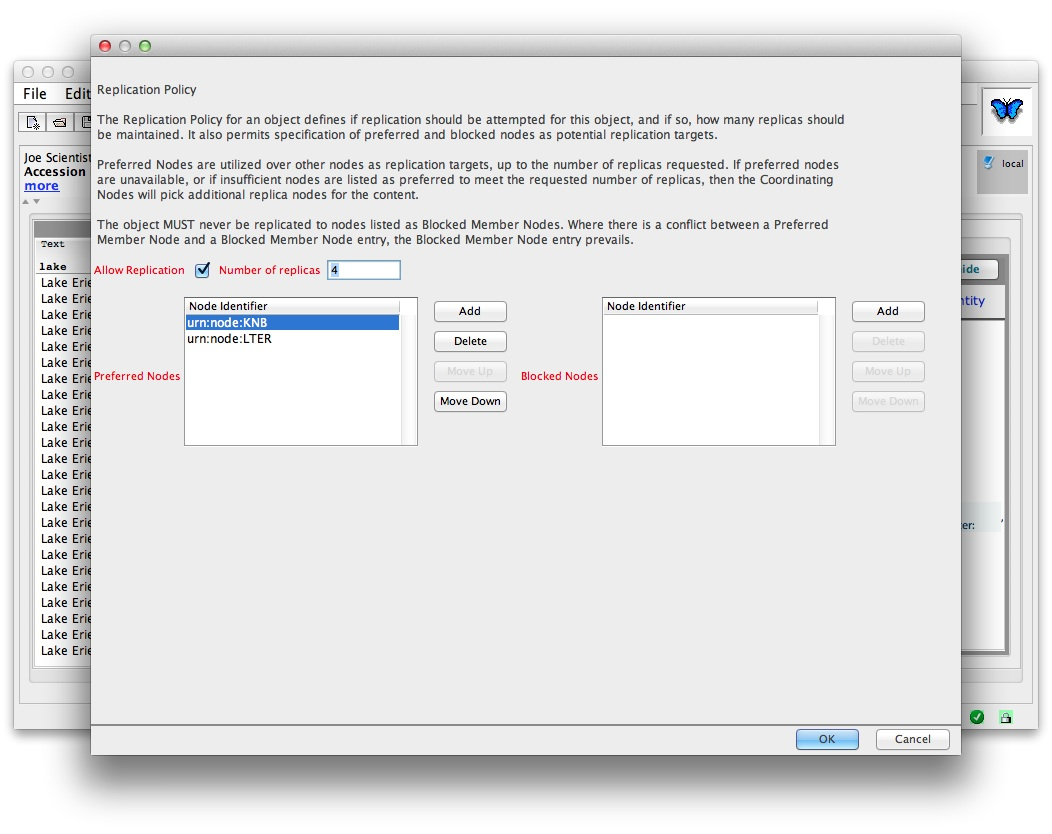
\includegraphics[width=0.7\textwidth]{images/wizard-dp-replication.jpg}
  \caption{Set the replication policy for a data package.}
  \label{fig:wizard-dp-replication}
\end{figure}

\subsubsection{Summary} \label{sec:wizard-dp-summary}

Step 15 of the Data Package Wizard (\autoref{fig:wizard-dp-summary})
confirms that you have entered the required documentation. Your data
package will be created when you click Finish. Note that you must save
the package, or the entered information will be lost.  See section 7 for
step-by-step instructions for adding data tables to your packages.

\begin{figure}
  \centering
    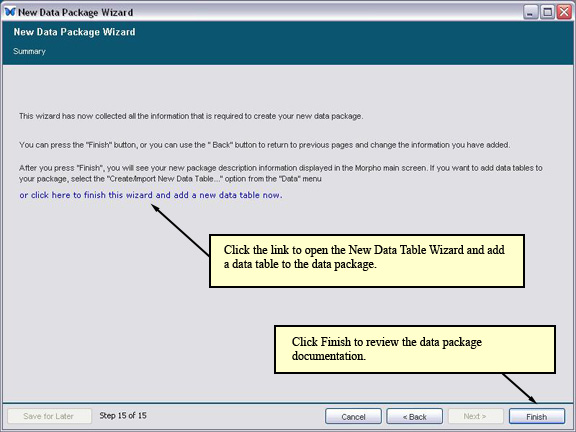
\includegraphics[width=0.7\textwidth]{images/wizard-dp-summary.jpg}
  \caption{The Summary screen.}
  \label{fig:wizard-dp-summary}
\end{figure}

Click Finish to view the data package documentation
(\autoref{fig:viewer-metadata}), or click the ``or click here to finish
this wizard and add a new data table now'' link to add a data table to
the package immediately.

If you have not already saved your package (File $>$ Save), Morpho will
prompt you to save the package before you close it. You can choose to
save the package locally and/or to the network. To edit the data package
documentation, use the options in the \nameref{sec:menu-documentation}.
For more information about editing package documentation, see
\nameref{sec:editing}.

\begin{figure}
  \centering
    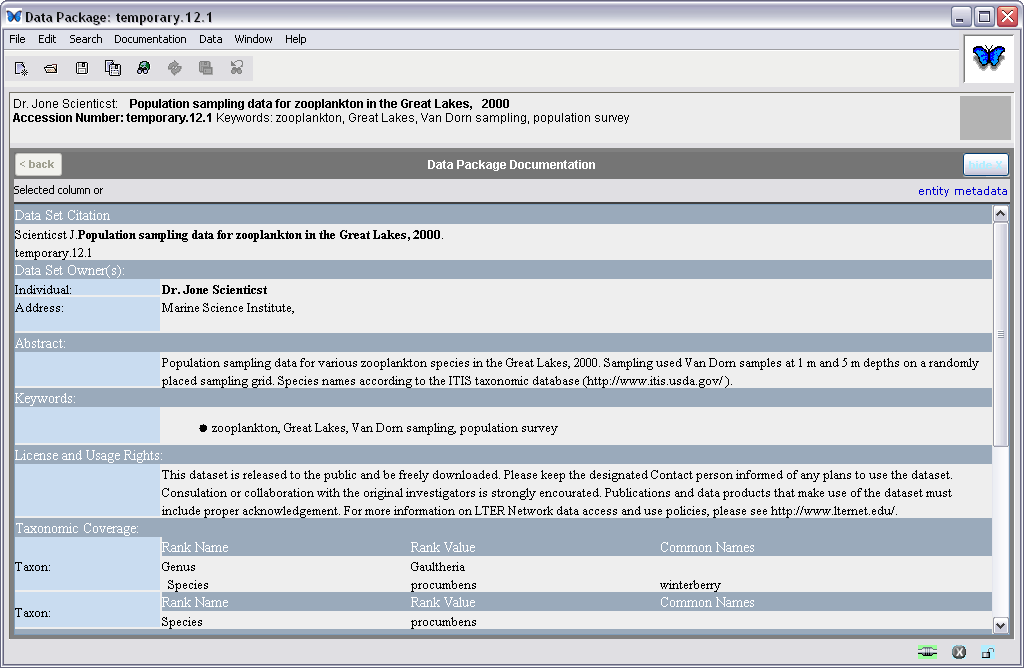
\includegraphics[width=0.7\textwidth]{images/viewer-metadata.png}
  \caption{Data package documentation is displayed by Morpho after the
    user clicks the Finish button.}
  \label{fig:viewer-metadata}
\end{figure}

\subsection{Saving Incomplete Data Packages} \label{sec:dp-saveforlater}

You can save an incomplete data packages during the New Package Wizard.
Click the ``Save for Later'' button at any step and the incomplete data
package will be saved locally (\autoref{fig:wizard-dp-saveforlater}).
The incomplete data package can be opened like any other data package
from the open menu option. After opening the incomplete data package,
Morpho will start the wizard at the last save point. When the wizard is
finished, a complete data package is saved.

\begin{figure}
  \centering
    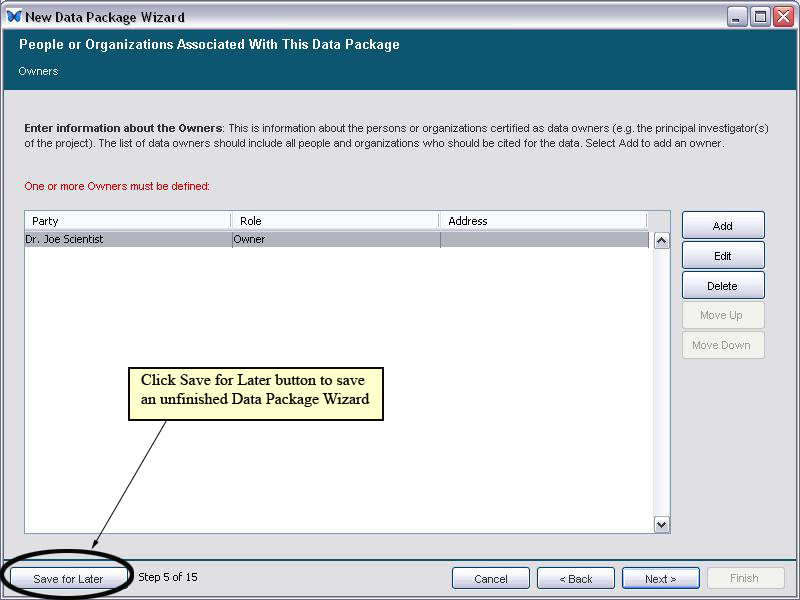
\includegraphics[width=0.7\textwidth]{images/wizard-dp-saveforlater.jpg}
  \caption{Save an incomplete data package.}
  \label{fig:wizard-dp-saveforlater}
\end{figure}

\subsection{Recovering Incomplete Data Packages} \label{sec:dp-recover}

Morpho can recover previously entered metadata if the New Data Package
Wizard fails before saving a complete data package. The next time Morpho
is launched, a window (\autoref{fig:dialog-open-recovered}) will show any
incomplete data packages that result from a failed wizard. The recovered
data packages can be opened and completed at this point. Choosing
``Cancel'' still allows the wizard to be completed later by opening the
data package from Morpho’s Open dialog.

\begin{figure}
  \centering
    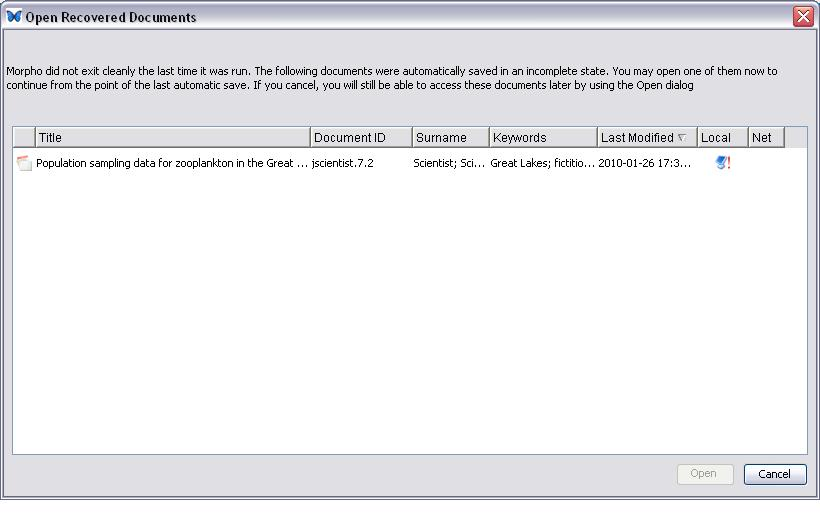
\includegraphics[width=0.7\textwidth]{images/dialog-open-recovered.jpg}
  \caption{Display the recovered data packages.}
  \label{fig:dialog-open-recovered}
\end{figure}
